\apendice{Plan de Proyecto Software}

\section{Introducción}

Se incluye a continuación la planificación seguida a lo largo de este proyecto: a nivel temporal, especificando las tareas realizas, a nivel económico, estimando un coste del trabajo, y de forma breve, a nivel legal, indicando los aspectos necesarios.

\section{Planificación temporal}

Para la planificación temporal de este proyecto, se ha estimado emplear la metodología Scrum, que consiste en un marco de trabajo para la gestión de proyectos, basado en un enfoque iterativo e incremental. El enfoque incremental se refiere a los sprints, ciclos de trabajo de duración fija que van delimitando las tareas del proyecto. Estas tareas han sido recogidas en GitHub en el apartado de issues, y la duración de los sprints comprende de. Por otro lado, el enfoque iterativo permite la mejora y el avance del proyecto, pues la creación continua de nuevos sprints implica haber alcanzado los objetivos del anterior. 

\clearpage
\textbf{Sprint 1} (10/03/2024 – 20/03/2024) 
\begin{enumerate}
    \item[-] \textit{Búsqueda de información}: conocimiento inicial sobre la dinámica glucosa insulina en el organismo, elementos biológicos implicados y mecanismos regulatorios.
    \item[-] \textit{Clasificación de los modelos dinámicos de la glucosa}: búsqueda bibliográfica de los modelos matemáticos que más se ajustan al comportamiento de la glucosa. Encontramos especial relevancia en los Modelos de Bergman y Ackerman, y estudiamos la posibilidad de incluir otras variantes de ellos.
\end{enumerate}

\begin{figure}[htbp]
    \centering
    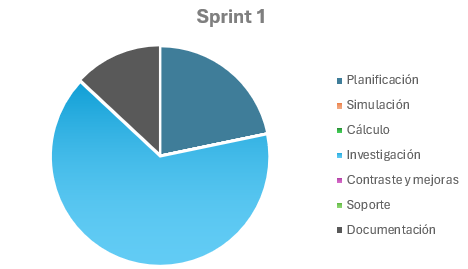
\includegraphics[width=0.8\linewidth]{img/Sprints/1.png}
    \caption{Sprint 1: Distribución de tareas.}
    \label{fig:sprint1}
\end{figure}

\textbf{Sprint 2} (20/03/2024-30/04/2024)
\begin{enumerate}
    \item[-] \textit{Modelado de los modelos matemáticos}: búsqueda exhaustiva de los sistemas de ecuaciones que rigen los modelos seleccionados. Comprensión de las variables y parámetros que los componen.
    \item[-] \textit{Modelo Mínimo de Bergman}: estudio del funcionamiento del modelo. Búsqueda de referencias bibliográficas que permitan comenzar las simulaciones. Reflejo del sistema glucorregulatorio óptimo.
    \item[-]  \textit{Modelo de Ackerman}: estudio del funcionamiento del modelo. Búsqueda de referencias bibliográficas por constituirse como el modelado pionero de la glucosa e insulina.
\end{enumerate}

\begin{figure}[htbp]
    \centering
    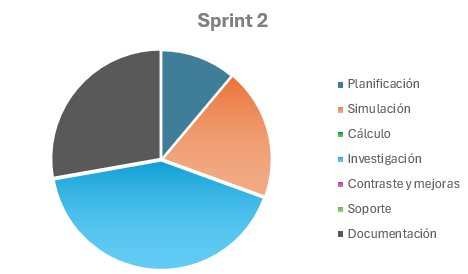
\includegraphics[width=0.8\linewidth]{img/Sprints/2.png}
    \caption{Sprint 2: Distribución de tareas.}
    \label{fig:sprint2}
\end{figure}


\textbf{Sprint 3} (30/03/2024 – 9/04/2024)
\begin{enumerate}
    \item[-] \textit{Formación en Latex}: búsqueda de información sobre el manejo en LaTex. Esta tarea comprende el aprendizaje de la inclusión de gráficas, ecuaciones, tablas, y otros elementos para el trabajo.
    \item[-] \textit{Búsqueda de datos experimentales}: puesta en contacto con el Servicio de Nutrición del Hospital de Burgos (HUBU). Búsqueda de datos de pacientes diabéticos y no diabéticos.
    \item[-]  \textit{Validación de los modelos con datos reales}: issue creado para estudiar el comportamiento de estos modelos con datos reales de pacientes, con la finalidad de observar las diferencias significativas entre ellos.
\end{enumerate}
\clearpage

\begin{figure}[htbp]
    \centering
    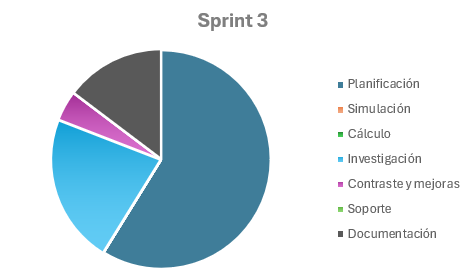
\includegraphics[width=0.8\linewidth]{img/Sprints/3.png}
    \caption{Sprint 3: Distribución de tareas.}
    \label{fig:sprint3}
\end{figure}

\textbf{Sprint 4} (9/04/2024-19/04/2024)
\begin{enumerate}
    \item[-] \textit{Obtención de datos}: anonimización y confidencialidad: Solicitud de datos anonimizados por parte del HUBU. Redacción y envío del Informe Bioético de Protección de Datos. No se ha podido completar esta tarea debido a que no se logró la obtención de los datos. 
    \item[-] \textit{Modelo de Bergman, ejercicio}: inclusión de la variable en el modelo y visualización de resultados iniciales para el comportamiento adecuado del sistema glucorregulatorio.
    \item[-]  \textit{Validación de los modelos con datos reales}: issue creado para estudiar el comportamiento de estos modelos con datos reales de pacientes, con la finalidad de observar las diferencias significativas entre ellos.
\end{enumerate}
\clearpage
\begin{figure}[htbp]
    \centering
    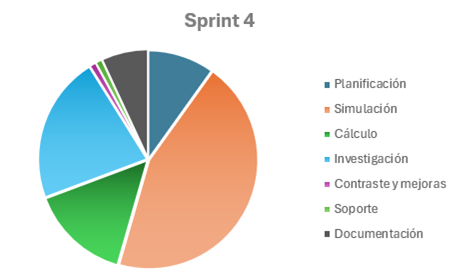
\includegraphics[width=0.8\linewidth]{img/Sprints/4.png}
    \caption{Sprint 4: Distribución de tareas.}
    \label{fig:sprint4}
\end{figure}

\textbf{Sprint 5} (19/04/2024- 29/04/2024)
\begin{enumerate}
    \item[-] \textit{Modelo de Berman Modificado}: revisión bibliográfica de artículos que incluyan otras ecuaciones que permitan modelar de forma más amplia el comportamiento de la glucosa. 
    \item[-] \textit{Insulina exógena}: inclusión de la entrada en el modelo, y estudio de su efecto para pacientes diabéticos.
    \item[-]  \textit{Modelo de Bergman Modificado y perturbaciones}: inclusión de otras variables, como son el ejercicio y la ingesta. Comparación de salidas obtenidas.
\end{enumerate}
\clearpage
\begin{figure}[htbp]
    \centering
    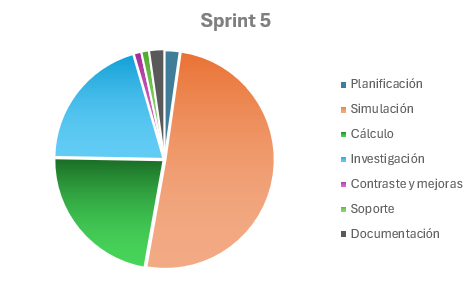
\includegraphics[width=0.8\linewidth]{img/Sprints/5.png}
    \caption{Sprint 5: Distribución de tareas.}
    \label{fig:sprint5}
\end{figure}

\textbf{Sprint 6} (29/04/2024- 9/05/2024)
\begin{enumerate}
    \item[-] \textit{Inclusión de la insulina variable y constante en el modelo}: simulación del Modelo de Bergman para una insulina variable, pues previamente se había considerado únicamente la variable.
    \item[-] \textit{Papel del páncreas en el sistema glucorregulatorio}: se estudia su mecanismo de acción en el organismo.
    \item[-]  \textit{Variación de los parámetros del modelo de Bergman}: se recogen varios análisis, entre los que destaca la tasa de eliminación de glucosa p1.
\end{enumerate}
\clearpage
\begin{figure}[htbp]
    \centering
    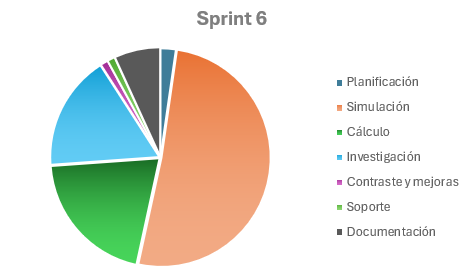
\includegraphics[width=0.8\linewidth]{img/Sprints/6.png}
    \caption{Sprint 6: Distribución de tareas.}
    \label{fig:sprint6}
\end{figure}

\textbf{Sprint 7} (9/05/2024-19/05/2024)
\begin{enumerate}
    \item[-] \textit{Insulina exógena y ejercicio físico}: una vez estudiadas las variables por separado, se combinan ambas para observar su efecto.
    \item[-] \textit{Insulina prolongada y rápida}: se considera el caso de intentar simular las diferentes acciones de la insulina. Se obtiene una estimación.
    \item[-]  \textit{Plan de ingesta completo.}
\end{enumerate}

\begin{figure}[htbp]
    \centering
    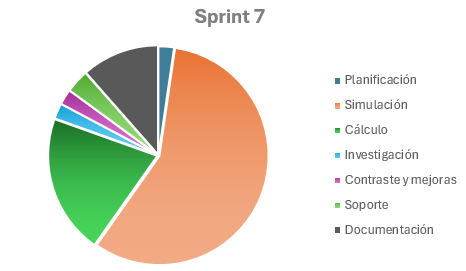
\includegraphics[width=0.8\linewidth]{img/Sprints/7.png}
    \caption{Sprint 7: Distribución de tareas.}
    \label{fig:sprint7}
\end{figure}
\clearpage
\textbf{Sprint 8} (19/05/2024-29/05/2024)
\begin{enumerate}
    \item[-] \textit{Regulador para la insulina, control continuo}: estudio de los mecanismos de control, y de su posible implementación para sustituir la administración manual de la insulina exógena.
\end{enumerate}

\begin{figure}[htbp]
    \centering
    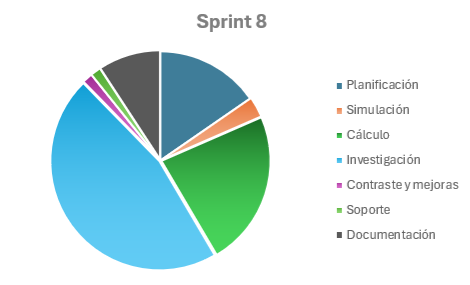
\includegraphics[width=0.8\linewidth]{img/Sprints/8.png}
    \caption{Sprint 8: Distribución de tareas.}
    \label{fig:sprint8}
\end{figure}

\textbf{Sprint 9} (29/05/2024-08/06/2024)
\begin{enumerate}
    \item[-] \textit{Regulador para el modelo de Berman modificado}: se sintonizan un par de reguladores, siguiendo diferentes métodos, para conseguir un control glucémico.
    \item[-] \textit{Latex, memoria y anexo}: se redacta de forma final los documentos, a partir de otros menores que se han ido redactando a lo largo del proyecto.
    \item[-]  \textit{Discusión de los resultados} una vez obtenidas todas las simulaciones llevadas a cabo en el estudio.
\end{enumerate}
\clearpage
\begin{figure}[htbp]
    \centering
    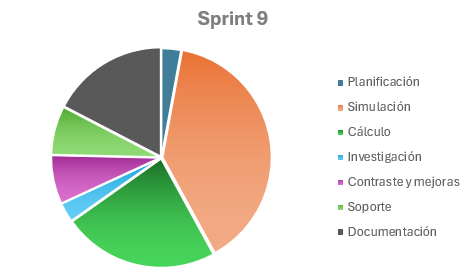
\includegraphics[width=0.8\linewidth]{img/Sprints/9.png}
    \caption{Sprint 9: Distribución de tareas.}
    \label{fig:sprint9}
\end{figure}

\textbf{Sprint 10} (08/06/2024-28/06/2024: Doble Sprint)
\begin{enumerate}
    \item[-]  \textit{Discusión de los resultados.} Ampliación de este issue con el fin de completar y orientar de manera más precisa el estudio. 
\end{enumerate}
\begin{figure}[htbp]
    \centering
    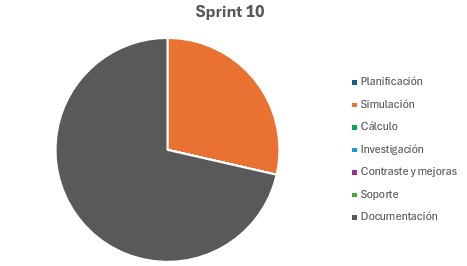
\includegraphics[width=0.8\linewidth]{img/Sprints/10.PNG}
    \caption{Sprint 10: Distribución de tareas.}
    \label{fig:sprint10}
\end{figure}
\clearpage
\section{Planificación económica}


Se indicarán para este apartado los costes tanto personales, como de materiales y desarrollo del proyecto.

Se comienza analizando el sueldo de un ingeniero promedio al salir de la carrera, obtenido en \cite{talent_com}\footnote{La conversión llevada a cabo se ha realizado con el calculador \cite{taxscouts}}:

\begin{table}[htbp]
    \centering
    \caption{Sueldo de un ingeniero en España y sus retenciones}
    \begin{tabular}{|c c|}
        \hline
        Sueldo bruto anual & 30000 \texteuro   \\
        Retenciones por IRPF & 4920 \texteuro \\
        Contribuciones a la Seguridad Social & 1935 \texteuro\\
        Tipo de retención & 16.40\% \\
        Sueldo neto anual & 23.145 \texteuro \\
        \hline
    \end{tabular}
    \label{tab:salario_ingeniero}
\end{table}

Tal y como se especifica para la elaboración del TFG, se estima el empleo de 360 horas en su realización, calculando el precio por hora. Se detallan en la Tabla \ref{tab:coste_personal} los costes personales para el proyecto \footnote{Datos obtenidos de la tabla anterior \ref{tab:salario_ingeniero}}.

\begin{table}[htbp]
    \centering
    \caption{Resumen de los costes personales para el proyecto.}
    \begin{tabular}{|c c|}
        \hline
        Sueldo al mes  & 1928,75 \texteuro   \\
        Sueldo por hora & 12,05 \texteuro \\
        Total por horas realizadas (360) & 4339,68 \texteuro\\
        \hline
    \end{tabular}
    \label{tab:coste_personal}
\end{table}

Se incluyen a continuación el resto de costes del proyecto a nivel material \footnote{Para más información de licencias de Office, entrar en \cite{microsoft}}. Se compone del coste del hardware (ordenador) y el software, que incluye la lincencia de Windows 10 Pro, el Paquete de Office, para redacción inicial de secciones así como elaboración de gráficos circulares, y la aplicación de Matlab, que contiene Simulink \footnote{Precios de Matlab: \cite{mathworks}.}.
\clearpage
\begin{table}[htbp]
    \centering
    \caption{Resumen de los costes materiales para el proyecto.}
    \begin{tabular}{|c c|}
        \hline
        Ordenador HP  & 698 \texteuro   \\
        Licencia Windows 10 Pro & 0 \texteuro (incluida) \\
        Paquete Office & 16,80 \texteuro\\
        Matlab y Simulink & 300 \texteuro\\
       Total material & 1014,8 \texteuro\\
        \hline
    \end{tabular}
    \label{tab:costes_mat}
\end{table}

Obteniendo un coste final:

\begin{table}[htbp]
    \centering
    \caption{Coste final del proyecto}
    \begin{tabular}{|c c|}
        \hline
       Costes personales  & 4339,68 \texteuro   \\
       Costes materiales & 1014,8 \texteuro \\
       \textbf{Total costes proyecto} & \textbf{5354,48} \texteuro\\
       \hline
    \end{tabular}
    \label{tab:costes_totales}
\end{table}

\section{Viabilidad legal}

Respecto a este apartado, siendo un estudio y al no haber empleado datos personales y reales de pacientes, simplemente hay que destacar: 
\begin{enumerate}
    \item[-] Programas de software abierto, como GitHub y Overleaf, no requieren de ninguna licencia específica. Para ambas se trabaja con la versión online, no siendo necesario llevar a cabo ninguna descarga ni asumir ningún coste para su uso.
    \item[-] Las licencias correspondientes al paquete Office requieren de contratación, que en este caso no ha sido necesaria por ser miembro de la Universidad de Burgos (UBU). Se diferencia por tanto la licencia académica y la comercial.
    \item [-] Respecto al programa más empleado para este estudio, MatLab, y su herramienta Simulink, requieren de una licencia para su uso, que en este caso no ha sido necesaria por el mismo motivo que en el apartado anterior. MATLAB y Simulink son productos de MathWorks y están sujetos a términos de uso específicos que se deben cumplir. Concretamente:
    \begin{enumerate}
        \item[-] Las licencias académicas de MATLAB, como es este caso, están diseñadas para ser utilizadas en actividades académicas, tales como la enseñanza, la investigación y el aprendizaje. Usos distintos a los mencionados no estan permitidos para esta modalidad. 
        \item [-] Estas licencias están limitadas a profesores, alumnos y figuras de la institución educativa determinadas. No está permitido el uso a personas ajenas a ellos.
        \item [-] No está permitido utilizar MatLab con licencia académica para desarrollar productos comerciales o realizar actividades lucrativas.
        \item[-] Está prohibida la distribución de sofware ni el uso a personas ajenas a la institución. 
    \end{enumerate}
\end{enumerate}
